% !TEX encoding = cp1250
\documentclass[a4paper,titlepage,11pt,twosides,floatssmall]{mwrep}
\usepackage[left=2.5cm,right=2.5cm,top=2.5cm,bottom=2.5cm]{geometry}
\usepackage[OT1]{fontenc}
\usepackage{polski}
\usepackage{amsmath}
\usepackage{amsfonts}
\usepackage{amssymb}
\usepackage{graphicx}
\usepackage{float}
\usepackage{url}
\usepackage{tikz}
\usepackage{multirow}
\usepackage{nicematrix}
\usetikzlibrary{arrows,calc,decorations.markings,math,arrows.meta}
\usepackage{rotating}
\usepackage[percent]{overpic}
\usepackage[cp1250]{inputenc}
\usepackage{xcolor}
\usepackage{colortbl}
\usepackage{pgfplots}
\usetikzlibrary{pgfplots.groupplots}
\usepackage{listings}
\usepackage{matlab-prettifier}
\usepackage{enumitem,amssymb}
\definecolor{szary}{rgb}{0.95,0.95,0.95}
\usepackage{siunitx}
\sisetup{detect-weight,exponent-product=\cdot,output-decimal-marker={,},per-mode=symbol,binary-units=true,range-phrase={-},range-units=single}
\SendSettingsToPgf
%konfiguracje pakietu listings
\lstset{
	backgroundcolor=\color{szary},
	frame=single,
	breaklines=true,
	tabsize=4,
%	numbers=left,
}
\lstdefinestyle{customlatex}{
	basicstyle=\footnotesize\ttfamily,
	%basicstyle=\small\ttfamily,
}
\lstdefinestyle{customc}{
	breaklines=true,
	frame=tb,
	language=C,
	xleftmargin=0pt,
	showstringspaces=false,
	basicstyle=\small\ttfamily,
	keywordstyle=\bfseries\color{green!40!black},
	commentstyle=\itshape\color{purple!40!black},
	identifierstyle=\color{blue},
	stringstyle=\color{orange},
}
\lstdefinestyle{custommatlab}{
	captionpos=t,
	breaklines=true,
	frame=tb,
	xleftmargin=0pt,
	language=matlab,
	showstringspaces=false,
	basicstyle=\footnotesize\ttfamily,
	%basicstyle=\scriptsize\ttfamily,
	keywordstyle=\bfseries\color{green!40!black},
	commentstyle=\itshape\color{purple!40!black},
	identifierstyle=\color{blue},
	stringstyle=\color{orange},
}

%wymiar tekstu (bez �ywej paginy)
\textwidth 160mm \textheight 247mm

%ustawienia pakietu pgfplots
\pgfplotsset{
tick label style={font=\scriptsize},
label style={font=\small},
legend style={font=\small},
title style={font=\small}
}

\def\figurename{Rys.}	
\def\tablename{Tab.}

%konfiguracja liczby p�ywaj�cych element�w
\setcounter{topnumber}{0}%2
\setcounter{bottomnumber}{3}%1
\setcounter{totalnumber}{5}%3
\renewcommand{\textfraction}{0.01}%0.2
\renewcommand{\topfraction}{0.95}%0.7
\renewcommand{\bottomfraction}{0.95}%0.3
\renewcommand{\floatpagefraction}{0.35}%0.5

\begin{document}
\frenchspacing
\pagestyle{uheadings}

%strona tytu�owa
\title{\bf Sprawozdanie z �wiczenia laboratoryjnego nr 1\vskip 0.1cm}
\author{Mateusz Palczuk}
\date{2022}

\makeatletter
\renewcommand{\maketitle}{\begin{titlepage}
\begin{center}{\LARGE {\bf
Wydzia� Elektroniki i Technik Informacyjnych}}\\
\vspace{0.4cm}
{\LARGE {\bf Politechnika Warszawska}}\\
\vspace{0.3cm}
\end{center}
\vspace{5cm}
\begin{center}
{\bf \LARGE Percepcja Maszyn \vskip 0.1cm}
\end{center}
\vspace{1cm}
\begin{center}
{\bf \LARGE \@title}
\end{center}
\vspace{2cm}
\begin{center}
{\bf \Large \@author \par}
\end{center}
\vspace*{\stretch{6}}
\begin{center}
\bf{\large{Warszawa, \@date\vskip 0.1cm}}
\end{center}
\end{titlepage}
}
\makeatother

\maketitle

\tableofcontents
% !TEX encoding = cp1250
\chapter{Wst�p}
W niniejszym sprawozdaniu opisany zosta� przebieg prac zwi�zanych z zadaniem laboratoryjnym nr 3.
Zadanie to polega�o na wykorzystaniu autokorelacji sygna�u do wyznaczenia t�tna z filmu.

Do realizacji zosta� wykorzystany jedynie pakiet MATLAB.
% !TEX encoding = cp1250

\chapter{Sygna�y zaszumione}
Program do generowania sygna�u zaszumionego, a nast�pnie jego odszumiania razem z komentarzami zosta� umieszczony poni�ej:

Stworzenie sygna�u oryginalnego z szumem:

\begin{lstlisting}
% Parametry systemu
Fs = 1000;     % Cz�stotliwo�� pr�bkowania [Hz]
T = 1/Fs;      % Okres pr�bkowania [s]
L = 2000;      % D�ugo�� sygna�u (liczba pr�bek)
t = (0:L-1)*T; % Podstawa czasu

% Przygotowanie sygna�u
N = 3;               % Liczba sinusoid w mieszaninie
A = [1.0   0.4  0.8] % Amplitudy kolejnych sinusoid
B = [ 15    27   83] % Cz�stotliwo�ci kolejnych sygna��w [Hz]
C = [  0 -pi/3 pi/7] % Przesuni�cia fazowe kolejnych sygna��w

x = zeros(size(t));
for i = 1:N
  x = x + A(i) * cos(2 * pi * B(i) * t + C(i));
end
x_orig = x;
x=x+randn(size(t))/3;
\end{lstlisting}

Wyznaczenie transformaty Fouriera i dostosowanie danych:

\begin{lstlisting}
Y = fft(x);     % transformata Fouriera

A = abs(Y);     % amplituda sygna�u
A = A/L;        % normalizacja amplitudy

A = A(1:L/2+1); % wyci�cie istotnej cz�ci spektrum
A(2:end-1) = 2*A(2:end-1);

F = angle(Y);   % faza sygna�u
F = F(1:L/2+1); % wyci�cie istotnej cz�ci spektrum

f_step = Fs/L;     % zmiana cz�stotliwo�ci
f = 0:f_step:Fs/2; % o� cz�stotliwo�ci do wykresu
\end{lstlisting}

Wykresy amplitudowy i fazowy:

\begin{lstlisting}
figure;
subplot(2, 1, 1)
plot(f, A);        % wykres amplitudowy
% figure;
subplot(2, 1, 2)
plot(f, F);        % wykres fazowy
\end{lstlisting}

Odtworzenie sygna�u z danych pozyskanych z transformaty Fouriera i narysowanie wykresu:

\begin{lstlisting}
odtw = zeros(size(t));
[maxA, maxI] = maxk(A, 3);
freq = maxI;
freq = freq - 1;
freq = freq/2;
maxA
maxI
freq
for i=1:3
    odtw = odtw + maxA(i) * cos(2 * pi * freq(i) * t + F(maxI(i)));
end

plot_size = 300;
figure; plot(x(1:plot_size));
hold on; plot(odtw(1:plot_size));
legend('Original with noise', 'Recreated');

figure; plot(x_orig(1:plot_size));
hold on; plot(odtw(1:plot_size));
legend('Original without noise', 'Recreated');
\end{lstlisting}

Wynik dzia�ania tego programu zosta� przedstawiony na rys.~\ref{no_noise} oraz rys.~\ref{with_noise}.
Jak �atwo zauwa�y� na rys.~\ref{no_noise} oba wykresy si� dok�adnie pokrywaj�.
Jest to spowodowane faktem, �e sygna� oryginalny sk�ada si� wy��cznie z trzech fali sinusoidalnych, wi�c je�eli odzyskamy ten sygna� przy pomocy r�wnie� trzech sinusoid otrzymamy dok�adnie ten sam sygna�. 

Sytuacja ma si� inaczej na rys.~\ref{with_noise} gdzie sygna� oryginalny zosta� zaszumiony.
Sygna� zosta� odzyskany z do�� dobr� dok�adno�ci�, ale nie jest to dok�adnie to samo. 

\begin{figure}
\centering
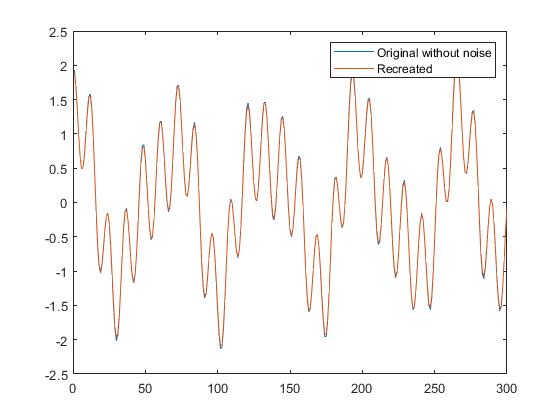
\includegraphics[width=1\textwidth]{dane/no_noise}
\caption{Sygna� odzyskany na�o�ony na sygna� oryginalny bez zaszumienia}
\label{no_noise}
\end{figure}

\begin{figure}
\centering
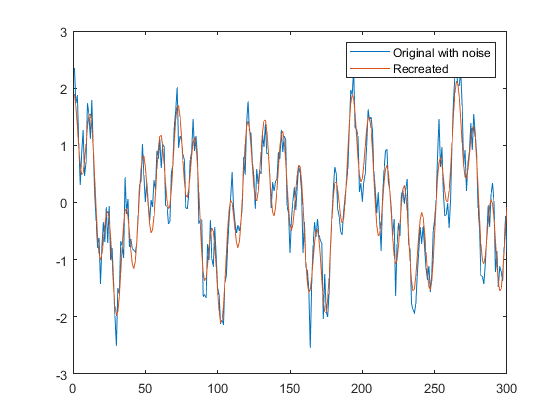
\includegraphics[width=1\textwidth]{dane/with_noise}
\caption{Sygna� odzyskany na�o�ony na zaszumiony sygna� oryginalny}
\label{with_noise}
\end{figure}

\chapter{Optyczny system pomiaru t�tna}
Do pomiaru t�tna zosta� wykorzystany film dostarczony przez prowadz�cego zaj�cia.
Nast�pnie film zosta� przerobiony na pojedyncze zdj�cia przy pomocy programu \verb|Adobe Media Encoder|.
Ca�y program zosta� przedstawiony razem z komentarzami poni�ej.

Wczytanie zdj��:

\begin{lstlisting}
% Liczba ramek do wczytania (przy 10 sekundach i 30 FPS b�dzie to 300)
N = 321;

% wektor jasno�ci
br = zeros(1, N);

% lista obraz�w do analizy
imds = imageDatastore('movie', 'FileExtension', '.jpg');

% alternatywnie mo�na za�adowa� bezpo�rednio plik wideo
% v = VideoReader('movie.mp4');

% wczytanie pierwszych N obraz�w i analiza jasno�ci
for i=1:N
    % wczytujemy obraz i przekszta�camy go do skali szaro�ci
    I = rgb2gray(imread(imds.Files{i}));
    % dla pliku wideo �adowanie ramki z otwartego �r�d�a
    % I = rgb2gray(read(v,i));

    % wyznaczamy �redni� z ca�ego obrazu
    br(i) = mean(I, 'all');
end
\end{lstlisting}

Przetworzenie danych z obraz�w:

\begin{lstlisting}
% dla u�atwienia p�niejszej analizy od razu mo�na odj�� od sygna�u sk�adow� sta��
br = br - mean(br);

% Parametry systemu
Fs = 30;     % Cz�stotliwo�� pr�bkowania [Hz]
T = 1/Fs;      % Okres pr�bkowania [s]
L = N;         % D�ugo�� sygna�u (liczba pr�bek)
t = (0:L-1)*T; % Podstawa czasu

x = br;
Y = fft(x);     % transformata Fouriera

A = abs(Y);     % amplituda sygna�u
A = A/L;        % normalizacja amplitudy

A = A(1:L/2+1); % wyci�cie istotnej cz�ci spektrum
A(2:end-1) = 2*A(2:end-1);

F = angle(Y);   % faza sygna�u
F = F(1:L/2+1); % wyci�cie istotnej cz�ci spektrum

f_step = Fs/L;     % zmiana cz�stotliwo�ci
f = 0:f_step:Fs/2; % o� cz�stotliwo�ci do wykresu
\end{lstlisting}

Narysowanie wykres�w i wyznaczenie t�tna w uderzeniach na minut�:

\begin{lstlisting}
figure;
subplot(2, 1, 1)
plot(f, A);        % wykres amplitudowy
subplot(2, 1, 2)
plot(f, F);        % wykres fazowy

[maxA, maxI] = maxk(A, 1);
bmp = f(maxI)*60

plot_size = 300;
figure; plot(br(1:plot_size));

\end{lstlisting}

Wynik tego programu zosta� przedstawiony na rys.~\ref{heart_rate} oraz zosta� wypisany w konsoli:

\begin{equation}
bmp = \num{67.2897}
\label{bmp}
\end{equation}

Jak wida� t�tno przedstawione na rys.~\ref{heart_rate} jest klarownie widoczne i mo�na by je zmierzy� nawet zliczaj�c przej�cia sygna�u przez 0.

R�wnie� t�tno zmierzone przy pomocy transformaty Fouriera (r�wnanie~\ref{bmp}) jest w pe�ni normalne, wi�c jest to wynik najpewniej poprawny.

Na rozdzielczo�� pomiaru sk�ada si� wy��cznie liczba klatek na sekund� zarejestrowanych w filmie.
W tym wypadku film mia� 30 klatek na sekund�, wi�c pomiar mia� rozdzielczo�� 30Hz.
Aby zwi�kszy� dok�adno�� pomiaru nale�a�oby nagra� film w wi�kszej liczbie klatek na sekund�.


\begin{figure}
\centering
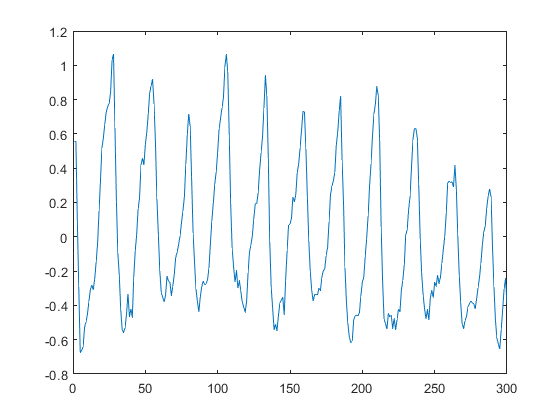
\includegraphics[width=1\textwidth]{dane/heart_rate}
\caption{Reprezentacja graficzna zmierzonego t�tna}
\label{heart_rate}
\end{figure}

\end{document}

